\documentclass[aspectratio=43,11pt]{beamer}
\usepackage[utf8]{inputenc}
\usepackage{caption}
\usepackage{makecell}
\usepackage{framed}
\usepackage{listings}
\usepackage{csquotes}
\usepackage{mathtools}
\usepackage{hyperref}
\usepackage{graphicx}   
\usepackage{amsmath,amssymb}
\usepackage[magyar]{babel}

\usetheme{realtimeweb}

\makeindex
\graphicspath{ {figs/} }

\lstdefinelanguage{JavaScript}{
  keywords={typeof, new, true, false, catch, function, return, null, catch, switch, var, if, in, while, do, else, case, break, await, async, const, let},
  keywordstyle=\color{blue}\bfseries,
  ndkeywords={class, export, boolean, throw, implements, import, this},
  ndkeywordstyle=\color{darkgray}\bfseries,
  identifierstyle=\color{black},
  sensitive=false,
  comment=[l]{//},
  morecomment=[s]{/*}{*/},
  commentstyle=\color{purple}\ttfamily,
  stringstyle=\color{red}\ttfamily,
  morestring=[b]',
  morestring=[b]"
}

\lstset{basicstyle=\ttfamily,
  showstringspaces=false,
  commentstyle=\color{red},
  keywordstyle=\color{blue}
}

\captionsetup[figure]{labelformat=original}
\setlength{\belowcaptionskip}{0.25cm}
\setlength{\abovecaptionskip}{0.25cm}

\definecolor{graycolor}{gray}{0.96}

\setbeamerfont{section number projected}{family=\rmfamily,series=\bfseries,size=\normalsize}
\setbeamercolor{section number projected}{bg=graycolor,fg=Blue}
\setbeamercolor*{item}{fg=Blue}
\setbeamercolor{block title}{fg=Blue,bg=graycolor}
\setbeamercolor{caption name}{fg=Blue}
\setbeamercolor{bibliography entry author}{fg=Blue}
\setbeamercolor{bibliography entry location}{fg=Blue} 
\setbeamercolor{bibliography entry note}{fg=Blue}  
\setbeamertemplate{footline}[frame number]
\setbeamertemplate{caption}[numbered]
\setbeamertemplate{navigation symbols} {} 
\setbeamertemplate{bibliography item}{\insertbiblabel}
\setbeamertemplate{footline}[frame number]
\setbeamertemplate{caption}[numbered]
\setbeamertemplate{frametitle continuation}{}

\title{Projekt Bemutató}
\subtitle{Community Space - A place for all your memos}
\author{Lukács Zsolt}

\begin{document}

\frame{\titlepage}

\section{Kollaboratív modell}

\begin{frame}{Kollaboratív modell}

    Tudásmegosztásra kihelyezett közösségi munkaplatform a vállalati/egyéb közösségen belüli gyors információmegosztásra és megőrzésre rövid memo-k formájában, ahol bárki könnyedén megoszthatja aktuális gondolatait/felhívásait/közléseit egy adott témáról.

    \medbreak

    Alapvető funkcionalitások és üzleti folyamatok:
    \begin{itemize}
        \item Felhasználók képesek kontókat létrehozni a platformhoz való csatlakozáshoz;
        \item Saját közösségeket, hub-okat létrehozni, meglévőkhöz csatlakozási kérelmeket leadni; tagokat adminisztrátor felhasználók menedzselhetik;
        \item Felhasználók képesek memo-kat megosztani különböző láthatósági szintekkel, prioritásokkal és határidővel kizárólag a hub-on belül, ezek elolvasni, módosítani, archívumba helyezni, törölni, kitűzni, teljesíteni, keresni közöttük, stb.;
        \item Felhasználók képesek megtekinteni milyen tevékenységek végződtek el a múltban interakciós listázással és átfogó képet kaphatnak az aktivitási hőtérképpel;
        \item Felhasználók képesek összegzés formájában megtekinteni az összes (már csatlakozott) hub-jukat, informálódni arról, hogy hány új memo van, hány aktív tag, hányan várakoznak a csatlakozásra, stb.;
        \item A felhasználók képesek az éppen aktív felhasználókat megtekinteni;
        \item A felhasználók értesítéseket kapnak a platformbéli érdekes eseményekről.
    \end{itemize}

\end{frame}
\section{Stratégiai modell}

\begin{frame}{Stratégiai modell}

    \begin{figure}[htbp]
        \centering
        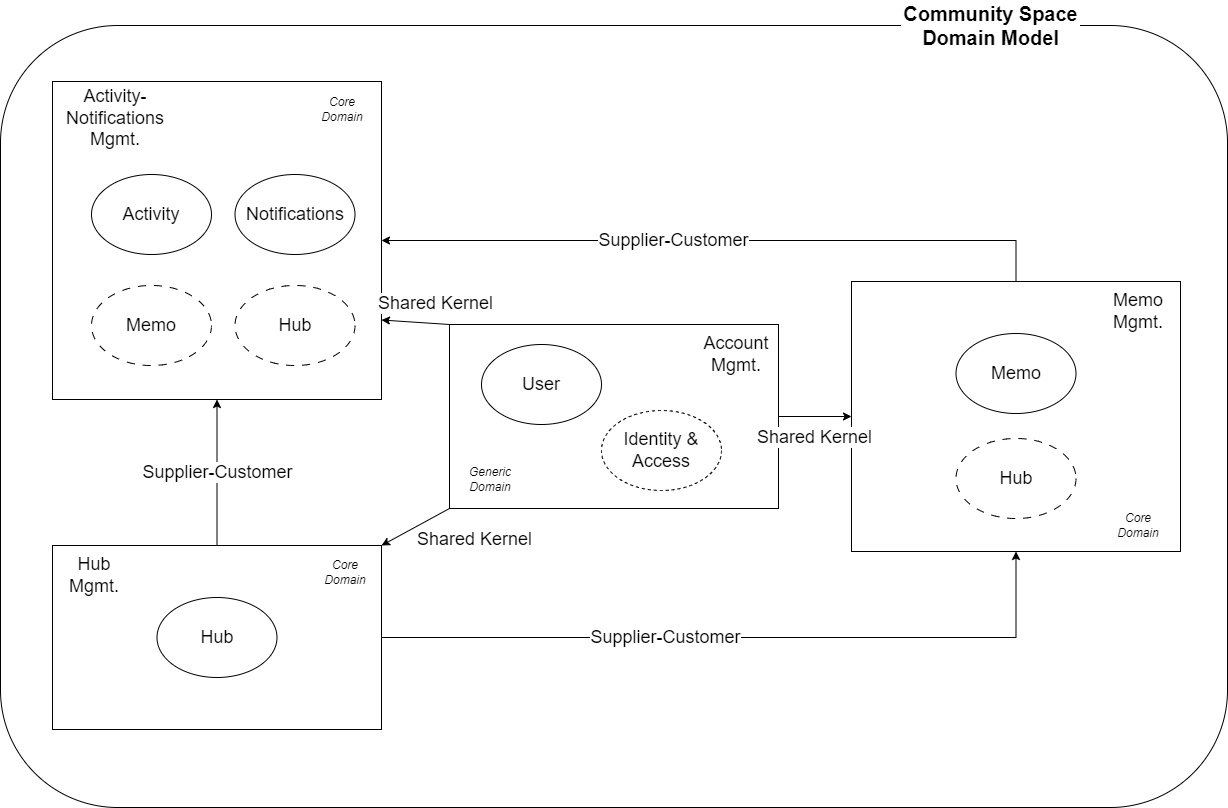
\includegraphics[width=0.98\textwidth]{strategic}
        \caption{CS domain modell}
    \end{figure}

\end{frame}
\section{Taktikai modell}

\begin{frame}{Taktikai modell}

    \begin{center}
        Rendszer alapvető központi entitásai: felhasználók, hub-ok, memo-k (kiegészítőleg aktivitások és értesítések).
    \end{center}

    \begin{figure}[htbp]
        \centering
        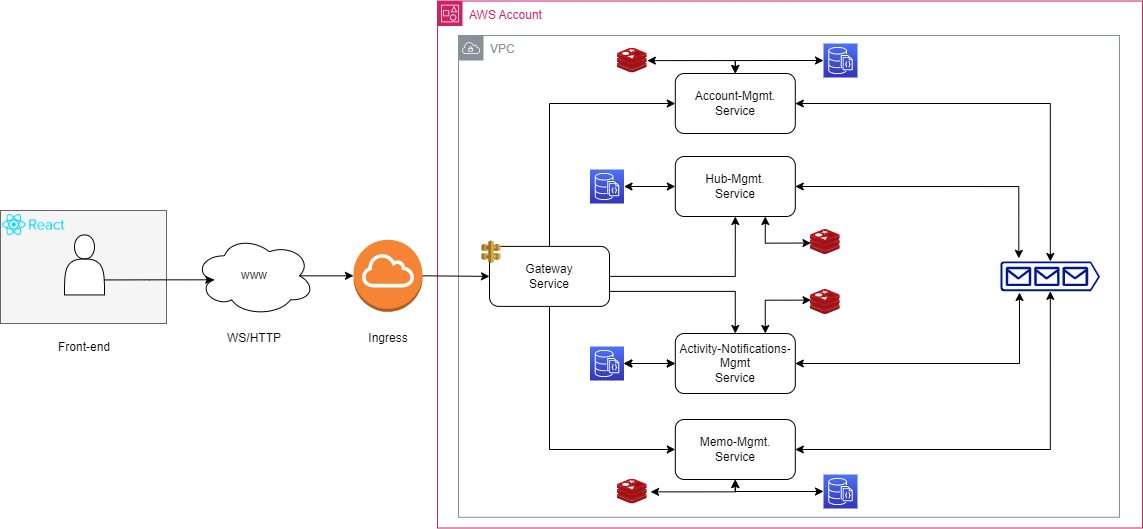
\includegraphics[width=0.98\textwidth]{arch}
        \caption{CS architektúra és komponens diagram}
    \end{figure}

    \begin{center}
        Micro-service architektúra összesen (jelenleg) 5 szolgáltatással.
    \end{center}

\end{frame}

\end{document}
